\section{Design}
\label{sec:design}

%In this section we begin with an explanation of live cloning to explain to the reader some the key challenges in designing a sandbox. 
%We then give a system overview of \texttt{Parikshan}, explaining each of its components. 
%Next, we explain how it inserts test cases, into the test harness, and finally we explain 
%how a user can use the \texttt{Parikshan} api to insert test cases in the test harness.

\begin{figure}[t]
  \begin{center}
    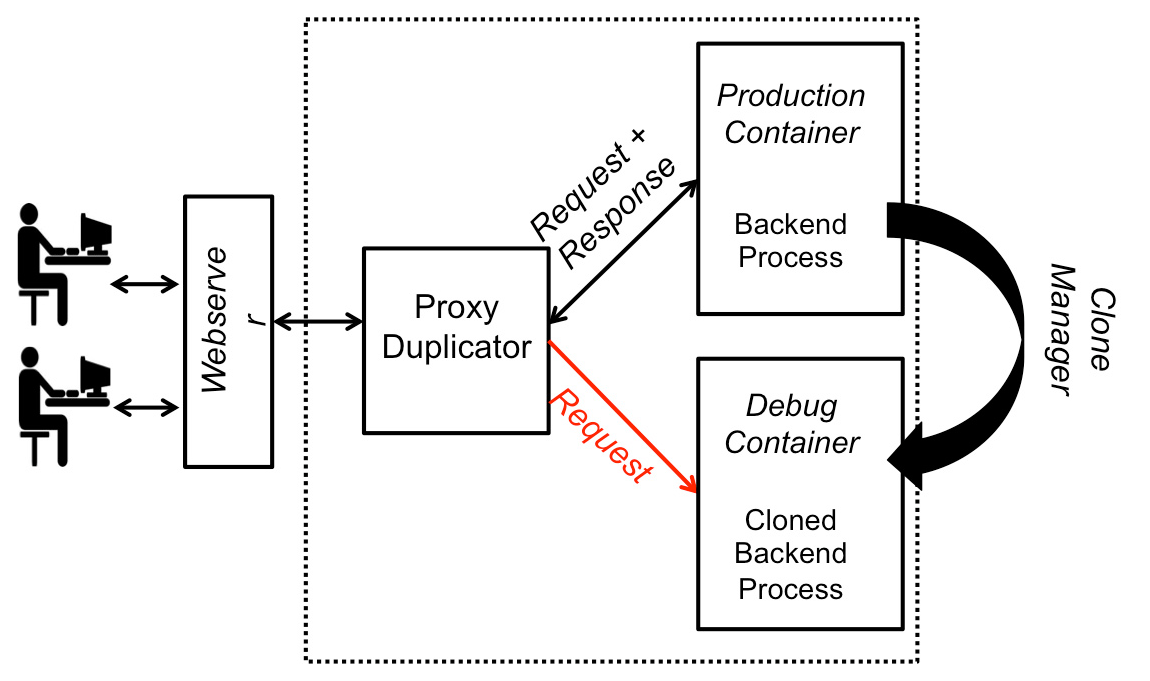
\includegraphics[width=0.5\textwidth]{figs/workflow2.eps}
    \caption{Backend wrapped around with Parakishan Run-time}
    \label{fig:workflow}
  \end{center}
\end{figure}

%\subsection{Workflow and Architecture}
%\label{sec:workflowArch}

%The basic workflow of \parikshan is as described in Figure \ref{fig:workflow}. 
%\parikshan can be applied at the boundary of every tier of a multi-tier system. 
%In figure \ref{fig:workflow} we show parikshan being applied to a single tier boundary 
%(communication from a webserver to a backend server) to showcase a simple example, 
%this process can be easily scaled depending on the complexity of the system design. 
%The architecture is driven by a proxy request duplication agent( see section \ref{ and a live clone manager.

\subsection{System Overview}
\label{sec:systemOverview}

Each instance of \parikshan can target only one tier at a time.
However, multiple instances can be orchestrated together especially when it's required for integration testing or cross tier results need to be correlated.
To begin with let us look at a simple example of client web-server with a database server as the backend (as shown in Figure \ref{fig:workflow}), where the test harness needs to be applied on the backend.
As explained earlier basic workflow of our system is to duplicate all network requests to the production backend server and a ``live cloned'' test container.
Traffic duplication is managed by our proxy network duplicator (see section \ref{sec:proxyDuplicator}), which uses several different strategies to clone user input to our test-container, with minimal impact on the production container.
Another core aspect of our design is how to implement ``live cloning''; this is the process by which a production container (in this case our backend service), can be cloned to create a test-container which has the same file system and process state. 
Cloning and syncing between the production container and the test-container is managed by our clone manager, which uses user-space containers OpenVZ and a variant of live migration to manage the cloning.
Next, we explain each of the modules in detail.
%The architecture can be divided into two parts: (1) A Proxy Network Duplicator, (2) container clone manager

%\begin{itemize} 

\subsection{Clone Manager} 
\label{sec:CloneManager}

\subsubsection{How does cloning work?}
\label{sec:cloning}

While the focus of our work is not to support VM Container migration, or to make changes to the hypervisor, we need to tweak the way typical hypervisors offer live migration for our purposes.
Before moving further we wish to clarify that instead of the standard live migration supported by hypervisors, \parikshan requires a cloning functionality. 
In contrast with live migration, where a container is copied to a target destination, and then the original container is destroyed, the cloning process requires both containers to be actively running, and be still attached to the original network.
This cloning requires some tweaking, and modification in both how compute migration is handled, and especially how the network migration is handled. 

To understand cloning in our context, let us understand how live migration works. 
Live migration refers to the process of moving a running virtual machine, guest os or container from one host node(physical machine) to another, without disconnecting any client or process running within the machine. 
Live migration is supported by most well known Hypervisors( vmware, virtualbox, xen, qemu, kvm) with different amount of efficiency.
There are several variants of migration, some of which require a short suspend time, while others are able to seamlessly transfer without any noticeable down-time by the user.
In general the process involves the following steps: 
(1) Firstly, the copy (\textit{rsync}) is initiated by a pre-copy memory migration, where the underlying hypervisor copies all the memory pages from the source to the destination. 
(2) Once pre-copy phase is finished, the VM is temporarily suspended, and all memory pages including live memory pages are transferred to the target node. 
Once all memory pages have been transferred the target container is restarted. 
Obviously, two rsync runs are needed, so the first one moves most of the data, while the container is still up and running, and the second one moves the changes made during the time period between the first rsync run and the VM stop
\footnote{Network migration is managed by the IAAS which publishes the same MAC address for the copied VM. 
Since the identity of the target container remains the same, the IAAS is able to give it same IP Address, and network traffic is rerouted after the identity is published in the network}.
%To reduce the down-time memory pages are transferred probabiliticly based on priority, and incase a page is not found a network fault is generated which executes a fetch from the original VM.

Instead of Live Migration, in Live Cloning, we do not suspend operations of the source container, rather we allow the container to keep executing in both production and test locations.
The more tricky aspect is that there are two containers with the same identities in the network and application domain. 
This is important, as the operating system and the process may be configured with the IP Address, or other networking operation, which cannot be changed without leading to a crash of the system.
Hence the same network identifier should map to two separate addresses.
Clearly the same ipAddress, mac addresses cannot be kept for both the production and test-container as that would lead to conflict in the network. 
There are two ways to resolve this : 
(1) Host each container behind their own network namespaces, on the same host machine, and configure packet forwarding to both containers such that the duplicator can communicate to them. 
Network namespaces(see internal mode, figure.\ref{fig:modesCloning}) is a definite possibility, and have been used by several hosting providers, to launch VM's with same private ipAddress, in a shared network domain \cite{OpenStack}. 
(2) Another approach is to host both containers in different machines with port forwarding setup to forward incoming TCP requests to containers behind a NAT (see external mode, figure.\ref{fig:modesCloning}). 
This is slightly more scalable and has clear separation of network and compute resources. 
However, an obvious downside to this approach is that it needs a new VM to be allocated.
This leads us to two different modes of implementation, which we discuss in the next section.

%As of now, we have implemented the second approach for our proof of concept mostly because of the ease of implementation.
%Further a packet level sniffer or mirror port would keep the same buffer and potentially timeout.
%To allow for some load-balancing and an application aware buffer, we went for a web application level proxy server to duplicate traffic to both containers. 
%Further in this section we explain how we deal with these challenges.

\subsubsection{Basic Design \& Modes}

The Clone Manager itself is just an interface which interacts with an \textit{agent} installed in each container host.
The clone manager dictates the frequency of cloning/syncing operations, as well as  coordinates setup operations/orchestration etc.
The agent itself is the driver for live cloning, and performs rsync operations, snapshot, transferring and starting the image.

\begin{figure}[t]
  \begin{center}
    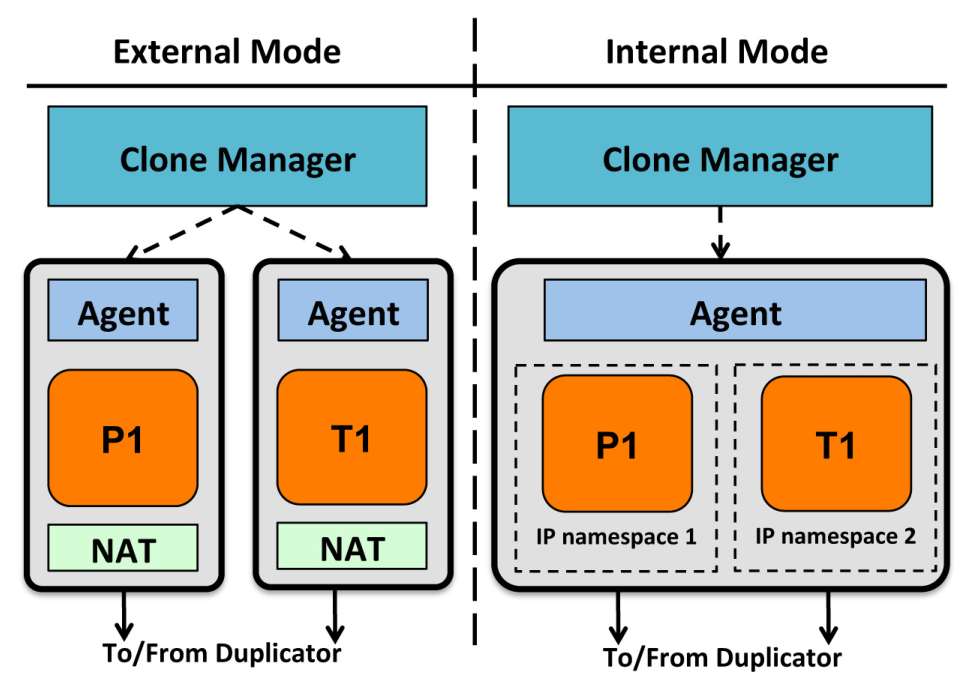
\includegraphics[width=0.5\textwidth]{figs/modesCloning.eps}
    \caption{External and Internal Mode for Live Cloning: P1 is the production container, and T1 is the test container, the Clone Manager interacts with an Agent which has drivers to implement live Cloning}
    \label{fig:modesCloning}
  \end{center}
\end{figure}


Test and production containers can be allocated in various schemes: we call these schemes \textit{modes}. 
Broadly speaking the clone manager works in 2 modes (see figure.\ref{fig:modesCloning}) : 
\begin{itemize}

\item \textit{Internal Mode}: In this mode we allocate the test-container and  production containers to the same host node. 
This would mean less suspend time, as the production container can be locally cloned ( instead of streaming over the network). 
Requires the same amount of resources as the original production container (number of host nodes remain the same), hence could potentially be cost-effective.
On the down-side, co-hosting the test and production containers, could have an adverse effect on the performance of the production container, hence effecting the user.
As we can see in figure.\ref{fig:modesCloning} the production container P1 and test container T1 are both hosted within the same physical host, and with the same ip addres, but their network is encapsulated within different network namespaces to sandbox them.
The duplicator is then able to communicate to both these containers with no networking conflict.

\item \textit{External Mode}: In this mode we provision an extra VM as the host of our test-container (this VM can host more than one test-containers), 
While this mechanism can have a higher overhead in terms of suspend time (~3 seconds, dependent on process state), and it will require provisioning an extra host-node, the advantage of this mechanism is that once cloned, the VM is totally separate and will not effect the performance of the production-container.
We believe that such a mode will be more beneficial in comparison to the internal mode, as testing is likely to be transient, and it is often more important to not effect user experience\footnote{ \textit{Scaled Mode}: This can be viewed as a variant of the External Mode, where we can scale out test-containers to several testing containers which can be used to do statistical testing and distribute the instrumentation load to capture the overhead easier. This reduces the frequency with which the container needs to be synced. This is currently out of the scope of this paper, however we aim to show this in a future publication.}.
As we can see in figure.\ref{fig:modesCloning} the production container P1 and test container T1, are hosted on two different host machines, and are encapsulated behind a NAT\cite{nat} (network address translator), hence they each have their ip's in an internal network thereby avoiding any conflict.

\end{itemize}

%\RestyleAlgo{boxruled}
%\LinesNumbered

%\\ \\
%\noindent \textbf{Implementation}\\

\subsubsection{Algorithm}

%The Clone Manager is responsible for creating a live running ``clone'' of the production container and launch it as the test-container. 
%In our current setup cloning is done for each target production environment in the same physical host machine 
%(we can clone to a different physical host as well, however for optimization purposes we have assumed that they will always be in the same local network).

In our current implementation, we are using OpenVZ\cite{openvz} as our container engine, and have modified the migration mechanism in vzctl \cite{vzctl} to make it work for live cloning instead. 
We tested this out on multiple VM's acting as host nodes for OpenVZ containers. 
To make the cloning easier and faster, we used OpenVZ's \textit{ploop} devices \cite{ploop} to host the containers. 
\textit{Ploop} devices are a variant of disk loopback devices where the entire file system of the container is stored as a single file. 
This makes features such as syncing, moving, snapshots, backups and easy separation of inodes of each container file system.

The algorithm for live cloning is explained below: 

\begin{algorithm}[ht]
\begin{algorithmic}
   \caption{Algorithm for Live Cloning using OpenVZ 
   \label{algCloning}}
 \begin{enumerate}
   \item Safety Checks(Checks that a destination server is available via ssh w/o entering a password, and version checking of OpenVZ running in it) 
   \item Runs rsync of container file system (\textit{ploop} device) to the destination server  
   \item Checkpoints and suspend the container 
   \item Runs a second rsync of the \textit{ploop} device to the destination  
   \item Start container locally 
   \item Set up port forwarding and packet duplication
   \item Starts the container on the destination 
  \end{enumerate}
\end{algorithmic}
\end{algorithm}

Let us imaging we are cloning production container C1 on Host H1 as test container C2 on Host H2. 
The initial setup requires certain safety checks and pre-setup to ensure easy cloning, these include: ssh-copy-id operation for accessing without password, checking pre-existing container ID's, check version of vzctl etc. 
These ensure that H1 and H2 are compatible, and ready for live-cloning.
Next, we run an intial rsync of container C1, from Host H1 to Host H2, this step does not require any suspension of C1, and copies the bulk of the container file system to the destination server (H2). 
The next step involves checkpointing, and dumping the process in memory state to a file, this is what allows the container to be restarted from the same checkpointed state. 
However for sanity of the container process, it is important to restart the container from the same file system state as it was when the checkpoint was taken.
To ensure this, we take a second rsync of the ploop device of C1, and sync it with H2, after this the original container can be restarted.
Next we copy the dump file from step 3, from H1 to H2, and resume a new container from that dump file.

The overhead of cloning depends on the I/O operations happening within the container between step 2 and step 4 (the first and the second rsync), as this will increase the number of dirty pages in the memory, which in turn will impact the amount of memory that needs to be copied during the suspend phase (as mostly the dirty bits at suspend time are those which were not committed to memory and hence need to be transferred).  
A few iteration of cloning a container back and forth between two OpenVZ instances ( on KVM's within the same physical machine), resulted in an average suspend time of 1.8 seconds for the production container, and 3.3 seconds for launch of the test-container
%( see table \ref{table:clonePerf}).
%add citation for OpenVZ Live Migration performance iteration testbed http://openvz.livejournal.com/47780.html
This is nearly the same as that of native live migration\cite{openvzLiveMigrationPerf}, and has lesser suspend time for the production container as we do not include the \textit{``copy dump file''}, or the \textit{``undump and resume phase''} for production containers. 
In section \ref{sec:performance}, we evaluate the performance of live cloning while doing increasing amount of random I/O write operations, as well as with doing page fetches  from webserver running the production container.

%The same amount of resources as the production container are reserved for the test-container. 
%After doing the pre-copy, we do a pause for syncing the two containers, and start them together. 
%Subsequent clone operations are optimized as they only require rsync for the change that has happened to the base image and in memory operation.
%After the intial setup, the frequency of cloning depends on the slowdown experienced by the test-container, and requirement of the test-case (some test cases may not require a long running test-window).

\iffalse

\begin{table}[t]
  \centering
    \begin{tabular}{ | p{2.2cm} | l | l | l | l | l | l | l |}
    \hline
    \textbf{Iteration} & \textbf{1} & \textbf{2} & \textbf{3} & \textbf{4} & \textbf{5} & \textbf{Avg} \\ \hline
    \textbf{Suspend + Dump} & 0.00 & 0.00 & 0.00 & 0.00 & 0.00 & 0.00\\ \hline
    \textbf{Pcopy after suspend} & 0.00 & 0.00 & 0.00 & 0.00 & 0.00 & 0.00\\ \hline
    \textbf{Copy Dump File} & 0.00 & 0.00 & 0.57 & 0.74 & 0.59 & 0.65\\ \hline
    \textbf{Undump and Resume} & 0.00 & 0.00 & 0.57 & 0.74 & 0.59 & 0.65\\ \hline
%    \textbf{--------------} & --- & --- & --- & --- & --- & --- & ---\\ \hline
    \textbf{Total Suspend Time} & 0.60 & 0.60 & 0.57 & 0.74 & 0.59 & 0.65\\ \hline
    \end{tabular}
\caption{Performance of Live Cloning (external mode) with a random file dump process running in the container}
\label{table:clonePerf}
\end{table}

\fi

\subsection{Proxy Network Duplicator} 
\label{sec:proxyDuplicator}

As described earlier an important aspect of live cloning is that we have two replicas which share the same identity. 
While we do not have strong consistency requirements for our production and test-container, in order for sandbox-testing to work, both containers must receive the same input.
This can be achieved in multiple ways, the easiest would be a port-mirroring mechanism either using software provided tap devices or in hardware switches (several vendors provide mirroring options). 
These are both pretty common, and are blackbox and do not require much configuration.
However, such port mirroring solution gives us minimal control on the traffic going to our test container.
The production and test-container may execute at varying speeds which will result in them being slightly out of sync.
Additionally we need to accept responses from both servers and drop all the traffic coming from the test-container, while still maintaining an active connection with the client.
Hence a layer 2 level network solution is not possible as some context of the address and state are required

Network proxies can be created at different levels in the network stack, for our purposes we have created a TCP proxy which mirrors the incoming traffic.
The TCP level duplicator is configured with the client facing ip address (hence it becomes a proxy), and essentially works as a socket reader/writer which reads incoming TCP streams and writes these streams to two different socket connections for the production and test containers.

\begin{figure}[t]
  \begin{center}
    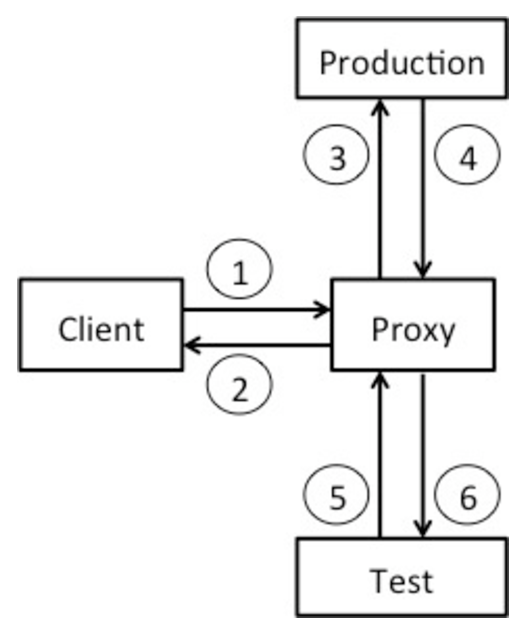
\includegraphics[width=0.45\textwidth]{figs/network_dup.eps}
    \caption{Description of the Network Duplicator. In \textit{synchronized} mode: there are 2 threads for each connection, Thread 1 executes steps [1,3,5], and Thread 2 executes [2,4,6] sequentially, hence the speed of packets sent to the production and the test container are synchronized. In \textit{asynchronous} mode, there are 4 threads for each connection, Thread 1 executes steps [1,3], Thread 2 executes [2,4], Thread 3 executes [5], and Thread 4 executes [6]. Hence communication to the test container and production container are asynchronous}
    \label{fig:duplicator}
  \end{center}
\end{figure}


\iffalse

\begin{figure}[t]
  \begin{center}
    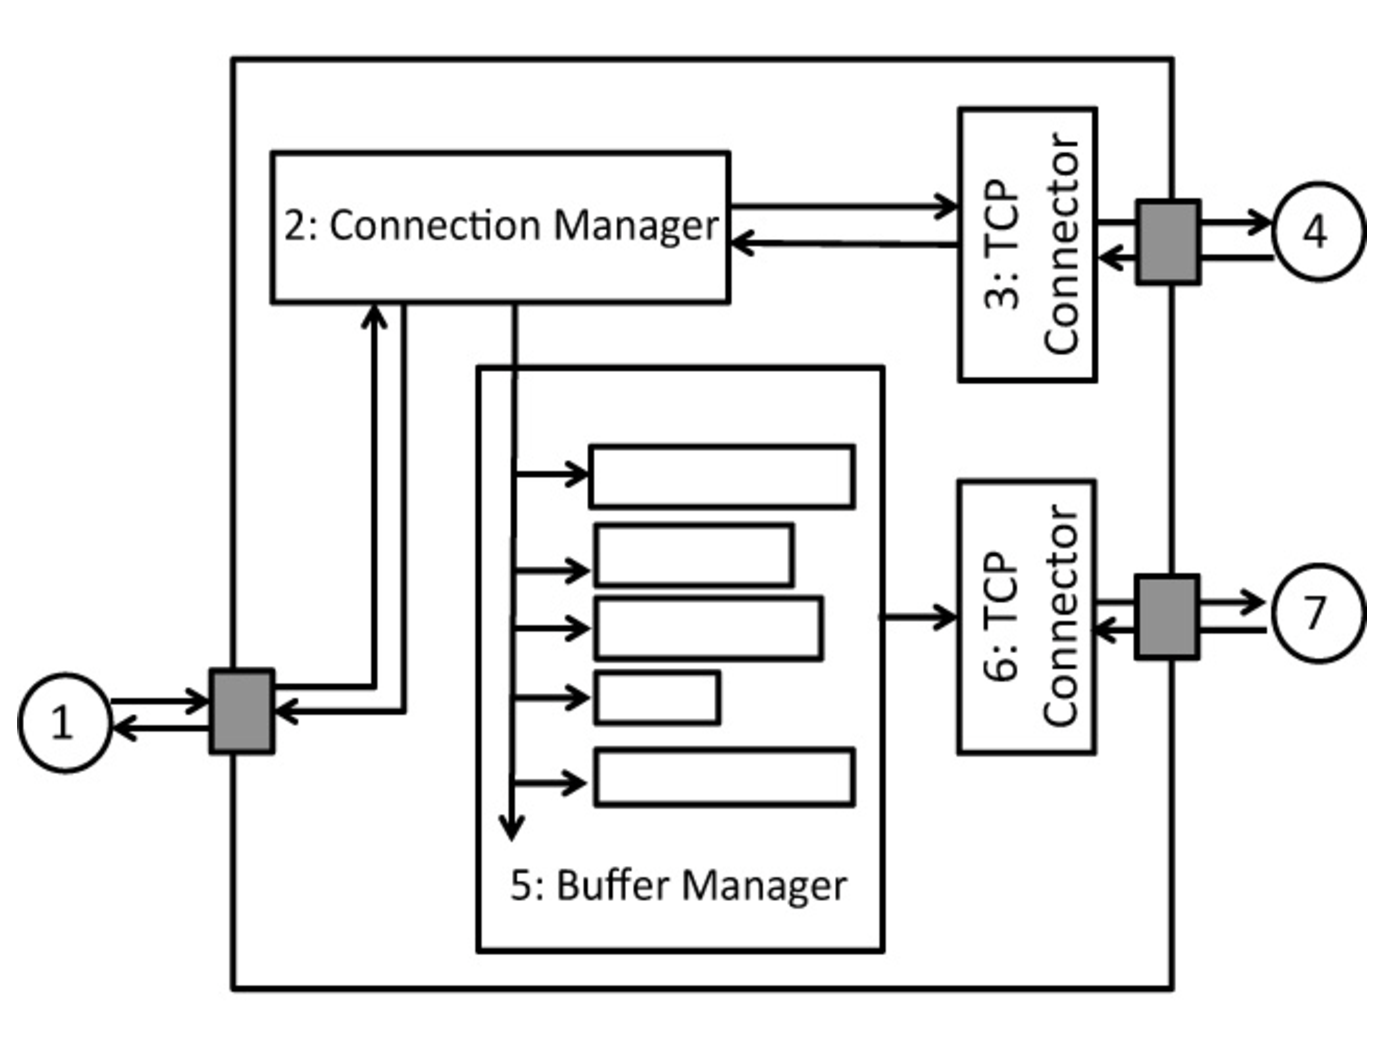
\includegraphics[width=0.5\textwidth]{figs/duplicator.eps}
    \caption{Description of the Network Duplicator}
    \label{fig:duplicator}
  \end{center}
\end{figure}

The workflow of each component is as follows: Traffic from the client (Node 1 in figure \ref{fig:duplicator}) is forwarded to the Connection Manager (Node 2 in figure \ref{fig:duplicator}). 
The connection manager essentially is a socket reader which copies, parses the incoming traffic. 
Based on the type of TCP request, a new connection is created or data is forwarded/received to/from the TCP Connector( Node 3, figure \ref{fig:duplicator}) which in turn creates a connection to actual production server.
In this way the connection manager and TCP connector follow the TCP state machine hence maintaining network packet sanity while forwarding traffic to the production container.
Simultaneously, the connection manager creates an internal copy of incoming traffic, and parses and sends it to the Buffer Manager (Node 5, figure \ref{fig:duplicator}).
\fi

In a naive scenario the connection could be simply forwarded to the test-container. 
However, it is likely that the rate of traffic consumption by the test-container is less than the production container. 
This means that the buffer size of the proxy for the test-container, the incoming client traffic and the amount of workload running on the test container will define the time window for which the test container will remain ``in-sync'' with the production container.

In this section we first discuss several strategies(we call modes) to design the duplication of traffic to the test container, and next we discuss briefly the ``testing window'' during which we believe that the test-container faithfully represents the execution of the production container. 

% ALGORITHM STYLE -- Released 8 April 1996
%    for LaTeX-2e
% Copyright -- 1994 Peter Williams
% E-mail Peter.Williams@dsto.defence.gov.au
\NeedsTeXFormat{LaTeX2e}
\ProvidesPackage{algorithm}
\typeout{Document Style `algorithm' - floating environment}

\RequirePackage{float}
\RequirePackage{ifthen}
\newcommand{\ALG@within}{nothing}
\newboolean{ALG@within}
\setboolean{ALG@within}{false}
\newcommand{\ALG@floatstyle}{ruled}
\newcommand{\ALG@name}{Algorithm}
\newcommand{\listalgorithmname}{List of \ALG@name s}

% Declare Options
% first appearance
\DeclareOption{plain}{
  \renewcommand{\ALG@floatstyle}{plain}
}
\DeclareOption{ruled}{
  \renewcommand{\ALG@floatstyle}{ruled}
}
\DeclareOption{boxed}{
  \renewcommand{\ALG@floatstyle}{boxed}
}
% then numbering convention
\DeclareOption{part}{
  \renewcommand{\ALG@within}{part}
  \setboolean{ALG@within}{true}
}
\DeclareOption{chapter}{
  \renewcommand{\ALG@within}{chapter}
  \setboolean{ALG@within}{true}
}
\DeclareOption{section}{
  \renewcommand{\ALG@within}{section}
  \setboolean{ALG@within}{true}
}
\DeclareOption{subsection}{
  \renewcommand{\ALG@within}{subsection}
  \setboolean{ALG@within}{true}
}
\DeclareOption{subsubsection}{
  \renewcommand{\ALG@within}{subsubsection}
  \setboolean{ALG@within}{true}
}
\DeclareOption{nothing}{
  \renewcommand{\ALG@within}{nothing}
  \setboolean{ALG@within}{true}
}
\DeclareOption*{\edef\ALG@name{\CurrentOption}}

% ALGORITHM
%
\ProcessOptions
\floatstyle{\ALG@floatstyle}
\ifthenelse{\boolean{ALG@within}}{
  \ifthenelse{\equal{\ALG@within}{part}}
     {\newfloat{algorithm}{htbp}{loa}[part]}{}
  \ifthenelse{\equal{\ALG@within}{chapter}}
     {\newfloat{algorithm}{htbp}{loa}[chapter]}{}
  \ifthenelse{\equal{\ALG@within}{section}}
     {\newfloat{algorithm}{htbp}{loa}[section]}{}
  \ifthenelse{\equal{\ALG@within}{subsection}}
     {\newfloat{algorithm}{htbp}{loa}[subsection]}{}
  \ifthenelse{\equal{\ALG@within}{subsubsection}}
     {\newfloat{algorithm}{htbp}{loa}[subsubsection]}{}
  \ifthenelse{\equal{\ALG@within}{nothing}}
     {\newfloat{algorithm}{htbp}{loa}}{}
}{
  \newfloat{algorithm}{htbp}{loa}
}
\floatname{algorithm}{\ALG@name}

\newcommand{\listofalgorithms}{\listof{algorithm}{\listalgorithmname}}



\subsubsection{Duplication Modes}
\label{sec:dupMode}

%\begin{enumerate}[leftmargin=*]
\begin{enumerate}[leftmargin=*]

\item \textbf{Synchronized Packet Forwarding Mode}

A naive strategy is to have a single worker thread to send and receive tcp stream to the production container as well as the test container.
This is the simplest strategy and is quite robust as far as sending proxy data is concerned. 
To understand this better let us look at figure \ref{fig:duplicator}: Here each incoming connection would be handled by 2 parallel threads in the proxy T1, and T2. 
Where T1 sends data from the client to the proxy (communication link 1), then sends data from proxy to production (link 3), and finally from proxy to test container (link 5). 
Whereas, thread 2 sends replies from production to proxy(link 4), then receives replies from test to proxy (link 6), which are then dropped. 
Thread T2 then forwards Packets received on link 4 are forwarded on link 2 to the client.

By design TCP is a connection oriented protocol and is designed for stateful delivery and acknowledgement that each packet has been delivered.
Packet sending and receiving are blocking operations by default, and hence if either the sender or the receiver is faster than the other the send/receive operations are automatically blocked or throttled.

In our case this can be viewed as follows: Let us assume that the client was sending packets at $X Mbps$ (link 1), and the production container was receiving/processing packets at $Y Mbps$ (link 3), where $Y<X$. 
Then automatically, the speed of link 1 and link 2 would be throttled to $Y Mbps$ per second, i.e the packet sending at the client would be throttled to accommodate the production server.
This behavior adheres to the default TCP protocol.
%, and if our proxy was only forwarding traffic to the production container it would be fine.
However, in the synchronized mode we also send packets to the test-container (link 5) in the same sequential thread T1. 
Hence if the speed of link 5 is $Z$ $Mbps$, where $Z < Y$, and $Z < X$, then the speed of link 1, and link 3 would also be throttled to $Z$ $Mbps$.

Such a communication model effects the user-experienced delay for the targeted SOA application, and is against the guiding principal of \parikshan.
To avoid the test-container to effect the communication between the client and the production server, we propose an asynchronous packet forwarding model discussed next.

%It especially works well with standard SOA architectures with small incoming packet flows, 
%as it means that the delay caused in the test and production container would be minimal.
%However, a major disadvantage of this approach is that every connection received would 
%finish a round trip connection with production container before sending the packets to the test-container.
%This would obviously delay all communication to the test-container by the amount of time it takes for the production container to respond. 
%However, more importantly it also effects the speed of the production container for every subsequent flow, 
%since it will have to wait for the time taken to send the packets to the test container.
%We assume a worker thread model for our proxy, where each connection is managed separately by one worker thread, 
%since our target is a service oriented architecture there should be frequent small connections from multiple users, hence a threading model is important.

\item \textbf{Asynchronous Packet Forwarding Model}

As shown in the previous section, in the synchronized mode the test container, can effect the speed of the production container as well. 
The main reason for this is because of blocking sends being used to forward packets from the client to the test-container and production container by the same sequential process.
In the asynchronous packet forwarding mode (see figure \ref{fig:duplicator}): we use 4 threads T1, T2, T3, T4 to manage each incoming connection to the proxy.
Thread T1 forwards packets from client to proxy (link 1), and from proxy to production container (link 2). 
It then uses a non-blocking send to forward packets to an internal pipe buffer shared between thread T1, and thread T3. 
Thread T3, then reads from this piped buffer and sends traffic forward to the test-container. 
Similarly Thread T2, receives packets from production container, and forwards them to the client, while Thread T4, receives packets from the test-container and drops them.

The advantage of this strategy is that any slowdown in the test-container will not effect the production container's communication as a non-blocking send is used to forward traffic to the production container. 
A side-effect of this strategy is that if the speed of the test-container is too slow compared to the production container, it may eventually lead to a buffer overflow. 
The time taken by a connection before which it overflows is called it's \emph{testing-window}.
We discuss the implications of the \emph{testing window} in section \ref{sec:window}.  
%In this strategy we have two worker threads which simultaneously handle sending and receiving tcp streams for the production container as well as the test container.
%Whenever any event happens the connection is established, and the incoming message is read to a buffer, this buffer is then sent to a worker thread for forwarding the data to the production container, and another thread for forwarding the data to the test container. 
%This means that unlike our previous model, the processing time of either the production container or the test container will not effect the performance of the other.
%We have a slightly modified worker thread model, in which each incoming connection is managed by two worker threads one for communication with the production and the other for the test.

\item \textbf{Asynchronous Load Balanced Packet Forwarding Model}

It is still possible that there will be slowdown, and a short packet window because of the overhead of running test-cases in the test container. 
This would mean that the test container will have a short time-window to execute test-cases.
To further increase this time window, we try and load balance testing across multiple test-containers, which can each get a duplicate copy of the incoming data. 
This would mean that there are multiple threads handling the incoming connection, one for the production container, and one for each of the test containers.
We believe that such a strategy would significantly increase the testing window size especially if the testing load is heavy.

\end{enumerate}

The algorithm for each of the packet forwarding modes has been described in Algorithm.\ref{algoDuplication}. 
%As an added explanation, the only difference between communication with the production container v/s the test container is that the when the proxy receives the message back from the production container, it sends the stream back to the client, on the other hand for the test container the packets are simply received and then dropped.


\iffalse

Since the speed of input from the client is not in sync production-container, we need to buffer incoming traffic and relay it to the the TCP Connector(Node 6, figure \ref{fig:duplicator}) as soon as the test-container is ready for new traffic. 
Since parallel connections can be initiated by the client on the same TCP port, the Buffer-Manager creates multiple buffers for each connection, and initiates new connections by following the same causal flow of the packets received from the client. 
Unlike record-replay systems \parikshan does not claim to have strong consistency requirements, and does not need to exactly follow the production container as the goal is not reproduce all non-determinism in the production environment, but instead capture input non-determinism, and complete system state from a given point of time.
We discuss consistency requirements further in section \ref{sec:consistency}

\fi

\subsection{Testing Window}
\label{sec:window}

At the time of the live cloning, the testing container has an identical status and receives the same input as the production container. 
Hence, any test-cases run in the testing container, should faithfully represent the status of the production container.
However, an obvious down-side to any debugging/testing is that it will add an overhead on the performance of the test-container as compared to the production environment.
%This would mean that the execution of requests in the test-container will lag behind the production container. 
To avoid this slowdown impacting the actual production container, we discussed an asynchronous forwarding strategy in section \ref{sec:dupModes}, where an unblocking send forwards traffic to a seperate thread which manages communication to the test-container. 
The thread has an internal buffer where all incoming requests are queued, the incoming request rate is dependent on how fast the production container manages the requests, where as the outgoing rate from the buffer is dependent on how fast the test-container processes the requests.
Depending on the workload, and the overhead induced in the test-container, can eventually lead to a buffer overflow. 
The time period till buffer overflow happens is called the testing-window.
For the duration of the testing-window, the test-container faithfully represents the production container as the testing-window of the test container. 
Once the buffer has overflown, the production container must be cloned again to ensure it has the same state.

In this section we try to model the testing window by using concepts well used in queuing theory(for the sake of brevity we will avoid going into too much detail, readers can find more about queueing theory models in \cite{queueWiki}).
The buffer overflow of our test-container can be modelled as a M/M/c/K queue (Kendall's notation\cite{kendall}), for our simplest asynchronous model, and as a M/M/c/K queue in the asynchoronous loadbalanced model.
An M/M/1/K queue, denotes a queue where requests arrive according to a poisson process with rate $\lambda$, that is the interarrival times are independent, exponentially distributed random variables with parameter $\lambda$ . 
The service times are also assumed to be independent and exponentially distributed with parameter $\mu$. Furthermore, all the involved random variables are supposed to be independent of each other. 
Further, the notation specifies that there are $c$ queues/ or alternatively $c$ servers managing the requests, and the queues is of a finite capacity, i.e. the queue can accommodate a maximum of K requests.
In our case $\lambda$ denotes the rate at which requests arrive to the buffer from the production container, and $\mu$ denotes the processing time overhead of each request in the test-container (to simplify the problem, we ignore the actual processing time of the test-container, as the incoming rate $\lambda$ is already synchronized with the production container processing time, and it is only the overhead added by the test-container which matters). 
In our simple asynchronous forwarding strategy, we have $c=1$ as we have only a single test-container, potentially as explained earlier, in a load-balanced asynchronous model this could be extended to $c$ servers to increase the time window.

Now based on this notation the expected size of the time window is :


%In queueing theory terms, the size of the testing window can be modelled as a special case of continuous-time Markov process also called the \emph{birth-death} process. 
%For the sake of brevity we will only briefly explain the basics of queueing theory

%It is possible that in heavy load conditions the buffers in the Buffer Manager may overflow. 
%Depending on the use-case the BufferManager can then trigger the CloneManager, which closes the analysis time-window and launches a fresh clone.
%Incoming traffic may potentially have a cumulative effect which will eventually lead to a buffer overflow in the BufferManager, hence leading to packet drops, and eventually leading to a modified state in the testing container, which can no longer faithfully represent the production container.
%This behavior is similar to packet dropping in classical TCP buffers, which rely on re-transmission of incoming packets from the client.
%However in our case if packets are dropped the client cannot re-transmit them as it not in sync with the test container.
%Hence in some cases \parikshan analysis, has to be restricted to a time-window dependent on the load of incoming traffic and the slowdown experienced by the test-container.

%Let the rate of incoming traffic be \lambda

\iffalse

\subsection{Network State Model}
\label{sec:networkStateModel}

Network communication in most applications consists of two core types of protocols: UDP \& TCP.
The UDP(User Datagram Protocol) allows the applications to send messages(referred to as datagrams) to other hosts in the network without prior communications to set up any transmission channels.
UDP uses a simple communication mechanism while minimizing protocols. 
It has no handshaking dialogues or acknowledgement of package delivery. It is broadly used for network traffic where speed is much more important than reliability (viz. network streaming applications like video etc.)
On the other hand TCP(Transmission Control Protocol) is a reliable error checked delivery stream.
It involves initially establishing the connection, and allowing for packet re-delivery or re-ordering to allow for reliable and dependable connection. 
While TCP is slower than UDP it is preferred for most normal connections between clients and server applications.

Since the UDP protocol has no error management mechanism, it automatically follows that machine state in a UDP connection is not important.
Hence in our design the duplicator can easily flood packets to the cloned UDP server by simply sending packets to the targeted host and port. 
Our solution for this is 

\fi
